% % !TEX program = pdflatex
% \documentclass{beamer}

% % \usetheme{Madrid}
% \usepackage{amsmath,mathrsfs}
% \usepackage{tikz}

\tikzset{elegant/.style={smooth,thick,samples=50,cyan}}
\tikzset{eaxis/.style={->,>=stealth}}

% \begin{document}
\begin{frame}
    \frametitle{Wasserstein Distance}
    \resizebox{\textwidth}{!}{
    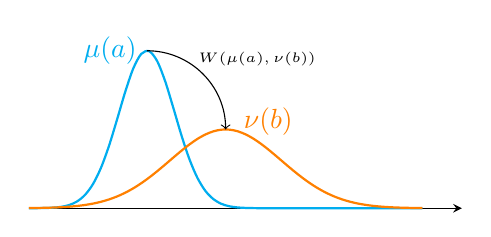
\begin{tikzpicture}
        % draw the axis
        \draw[eaxis] (-1.5,0) -- (4,0);
        % draw the function (piecewise)
        \draw[elegant,domain=-1.5:3.5] plot(\x,{pow(e,-(\x)^2*4)*2}) node [anchor=east] at (0,2) {$\mu(a)$};
        \draw[elegant,orange,domain=-1.5:3.5] plot(\x,{pow(e,-(\x-1)^2)}) node [anchor=west] at (1.1,1.1) {$\nu(b)$};
        
        \draw[->] (0,2) to[out=0, in=90] (1,1);
        \node at (1.4,1.9)  {\tiny$W(\mu(a),\nu(b))$};
    \end{tikzpicture}
    }
    \begin{center}
        Minimal effort transporting mass form $\mu$ to $\nu$
    \end{center}
\end{frame}
\begin{frame}
    \frametitle{Wasserstein Distance}
    \resizebox{\textwidth}{!}{
    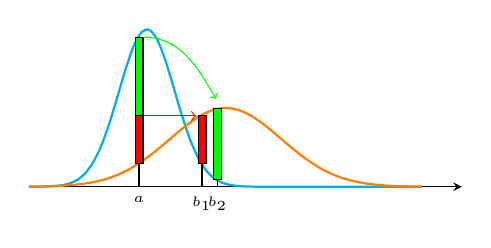
\begin{tikzpicture}
        % draw the axis
        \draw[eaxis] (-1.5,0) -- (4,0);
        % draw the function (piecewise)
        \draw[elegant,domain=-1.5:3.5] plot(\x,{pow(e,-(\x)^2*4)*2});
        \draw[elegant,orange,domain=-1.5:3.5] plot(\x,{pow(e,-(\x-1)^2)});
        
        \draw[fill=red] (-0.15,0.3) rectangle (-0.05,0.9) node [anchor=east] (block1) {};
        \draw[fill=green] (-0.15,0.9) rectangle (-0.05,1.9) node [anchor=east] (block2) {};
        \draw[fill=red] (0.65,0.3) rectangle (0.75,0.9) node (block3) {};
        \draw[fill=green] (0.85,0.09) rectangle (0.95,0.99) node (block4) {};
        
        \draw (-0.1,0.3) -- (-0.1,0) node [anchor=north] {\tiny$a$};
        \draw (0.7,0.3) -- (0.7,0) node [anchor=north] {\tiny$b_1$};
        \draw (0.9,0.1) -- (0.9,0) node [anchor=north] {\tiny$b_2$};
        
        \draw[red,->] (block1) -- (block3);
        \draw[green,->] (block2) to[out=0, in=120] (block4);
    \end{tikzpicture}
    }
    \begin{center}
        the transport plan from $a$ to $b$ is described by $\pi(a, b)$
    \end{center}
\end{frame}

\begin{frame}
    \frametitle{Wasserstein Distance}
    \resizebox{\textwidth}{!}{
    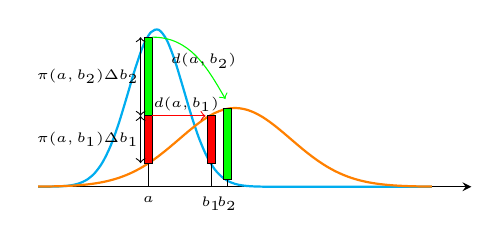
\begin{tikzpicture}
        % draw the axis
        \draw[eaxis] (-1.5,0) -- (4,0);
        % draw the function (piecewise)
        \draw[elegant,domain=-1.5:3.5] plot(\x,{pow(e,-(\x)^2*4)*2});
        \draw[elegant,orange,domain=-1.5:3.5] plot(\x,{pow(e,-(\x-1)^2)});
        
        \draw[fill=red] (-0.15,0.3) rectangle (-0.05,0.9) node [anchor=east] (block1) {};
        \draw[<->] (-0.2,0.3) -- (-0.2,0.9);
        \node [anchor=east] at (-0.1,0.6) {\tiny$\pi(a,b_1)\Delta b_1$};
        \draw[fill=green] (-0.15,0.9) rectangle (-0.05,1.9) node [anchor=east] (block2) {};
        \draw[<->] (-0.2,0.9) -- (-0.2,1.9);
        \node [anchor=east] at (-0.1,1.4) {\tiny$\pi(a,b_2)\Delta b_2$};
        \draw[fill=red] (0.65,0.3) rectangle (0.75,0.9) node (block3) {};
        \draw[fill=green] (0.85,0.09) rectangle (0.95,0.99) node (block4) {};
        
        \draw (-0.1,0.3) -- (-0.1,0) node [anchor=north] {\tiny$a$};
        \draw (0.7,0.3) -- (0.7,0) node [anchor=north] {\tiny$b_1$};
        \draw (0.9,0.1) -- (0.9,0) node [anchor=north] {\tiny$b_2$};
        
        \draw[red,->] (block1) -- (block3);
        \node at (0.38,1.05)  {\tiny$d(a,b_1)$};
        \draw[green,->] (block2) to[out=0, in=120] (block4);
        \node at (0.6,1.6)  {\tiny$d(a,b_2)$};
    \end{tikzpicture}
    }
\begin{equation*}
    \begin{aligned}
        &mass: \pi(a,b)\Delta a\Delta b \ \ \  path: d(a, b) \\
        &\Delta W={\color{red}\pi(a,b_1)\Delta a\Delta b_1}d(a,b_1) + {\color{green}\pi(a,b_2)\Delta a\Delta b_2}d(a,b_2) \\
    \end{aligned}
\end{equation*}
\pause
\begin{equation*}
    \begin{aligned}
        \hspace{-4mm}&W(\mu(a),\nu(b))|_{\pi=\pi(a,b)} = \iint \pi(a,b)d(a,b)\mathrm{d}a\mathrm{d}b = \int d(a,b)\mathrm{d}\pi(a,b)\\
    \end{aligned}
\end{equation*}
\end{frame}
\begin{frame}
    \frametitle{Wasserstein Distance}
    \resizebox{\textwidth}{!}{
    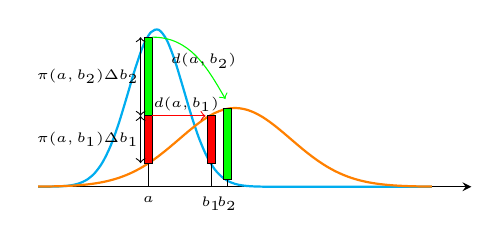
\begin{tikzpicture}
        % draw the axis
        \draw[eaxis] (-1.5,0) -- (4,0);
        % draw the function (piecewise)
        \draw[elegant,domain=-1.5:3.5] plot(\x,{pow(e,-(\x)^2*4)*2});
        \draw[elegant,orange,domain=-1.5:3.5] plot(\x,{pow(e,-(\x-1)^2)});
        
        \draw[fill=red] (-0.15,0.3) rectangle (-0.05,0.9) node [anchor=east] (block1) {};
        \draw[<->] (-0.2,0.3) -- (-0.2,0.9);
        \node [anchor=east] at (-0.1,0.6) {\tiny$\pi(a,b_1)\Delta b_1$};
        \draw[fill=green] (-0.15,0.9) rectangle (-0.05,1.9) node [anchor=east] (block2) {};
        \draw[<->] (-0.2,0.9) -- (-0.2,1.9);
        \node [anchor=east] at (-0.1,1.4) {\tiny$\pi(a,b_2)\Delta b_2$};
        \draw[fill=red] (0.65,0.3) rectangle (0.75,0.9) node (block3) {};
        \draw[fill=green] (0.85,0.09) rectangle (0.95,0.99) node (block4) {};
        
        \draw (-0.1,0.3) -- (-0.1,0) node [anchor=north] {\tiny$a$};
        \draw (0.7,0.3) -- (0.7,0) node [anchor=north] {\tiny$b_1$};
        \draw (0.9,0.1) -- (0.9,0) node [anchor=north] {\tiny$b_2$};
        
        \draw[red,->] (block1) -- (block3);
        \node at (0.38,1.05)  {\tiny$d(a,b_1)$};
        \draw[green,->] (block2) to[out=0, in=120] (block4);
        \node at (0.6,1.6)  {\tiny$d(a,b_2)$};
    \end{tikzpicture}
    }
    Choosing the best transportaion $\pi(a,b) \in \Pi(\mu,\nu)$:
\begin{equation*}
    \begin{aligned}
        \mathrm{Wasserstein}(\mu(a),\nu(b)) &= \inf_{\pi \in \Pi(\mu,\nu)} W(\mu(a),\nu(b))|_{\pi=\pi(a,b)} \\
        &=\inf_{\pi \in \Pi(\mu,\nu)}\int d(a,b)\mathrm{d}\pi(a,b)\\
    \end{aligned}
\end{equation*}
\end{frame}   
% \end{document}
%         % 建立相对坐标系
%         % \draw[help lines,xstep=.1,ystep=.1] (-1.5,0) grid (pi,2);